% ---------------------------------------------------------------------------
\section{Evaluating lookout with other anomaly detection methods}\label{sec:compareWithOtherMethods}
% ---------------------------------------------------------------------------

\subsection{Experiment 5: Normal distributions moving out in each iteration}
Non-outlier distribution: Normal 400 data points in $\mathbb{R}^6$ with mean 0 and sd 1 \\
Outlier distribution: 5 points normally distributed. In 5 dimensions they are similarly distributed as non-outlying points. In the other dimension they have mean $2 + (i-1)*0.5$ for $i \in \{1, \ldots, 10\}$ with sd = 0.2. \\
In each iteration the anomalous points get further away from the rest. Each iteration is repeated 10 times.

\begin{figure}[!ht]
	\centering
	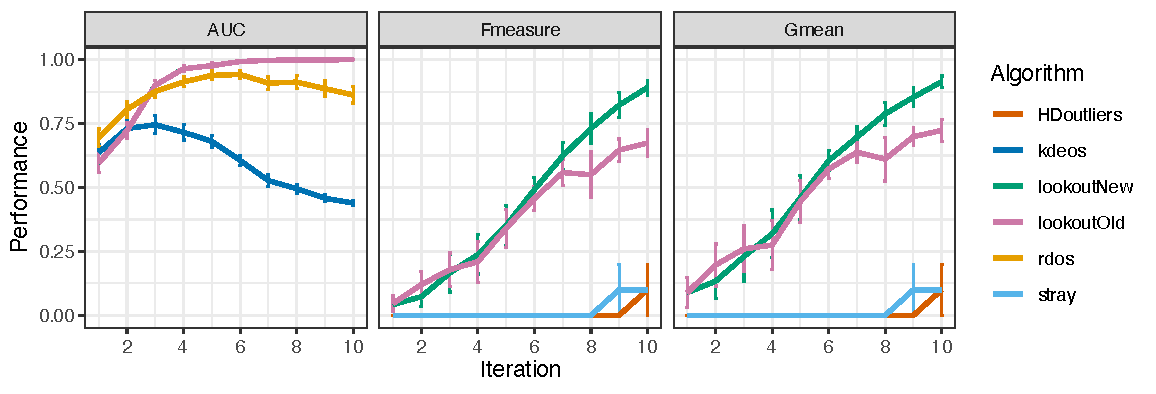
\includegraphics[width=\linewidth]{Figures/Experiment5_Comparison.pdf}
	\caption{Experiment 5 results}
	\label{fig:comparisonExp5}
\end{figure}


\subsection[Experiment 6: Annulus in R4]{Experiment 6: Annulus in $\mathbb{R}^4$}
Non-outlier distribution: 800 points distributed in an annulus in $\mathbb{R}^4$.  \\
Outlier distribution: 5 points moving in to the annulus in each iteration.
\begin{figure}[!ht]
	\centering
	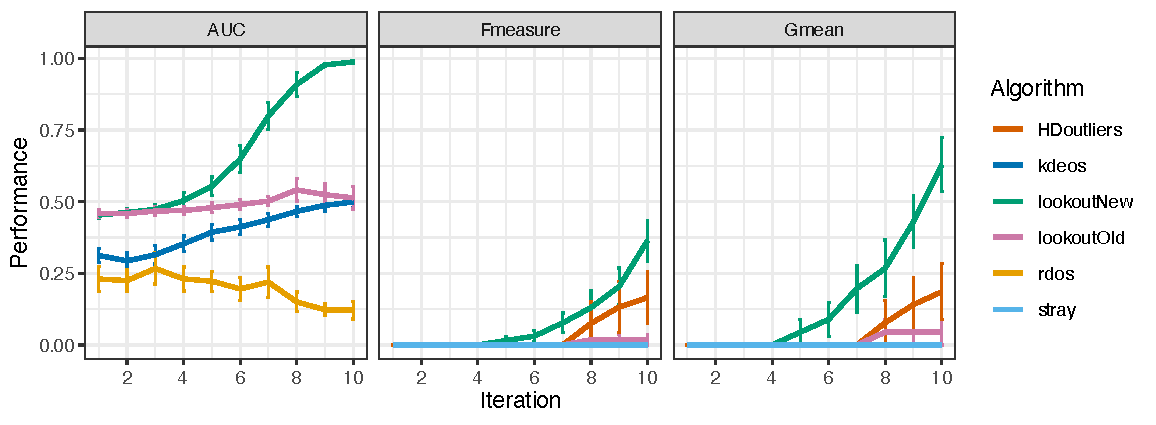
\includegraphics[width=\linewidth]{Figures/Experiment6_Comparison.pdf}
	\caption{Experiment 6 results}
	\label{fig:comparisonExp6}
\end{figure}


\subsection[Experiment 7: Unit cube in R20]{Experiment 7: Unit cube in $\mathbb{R}^{20}$}

Non-outlier distribution: Uniformly distributed unit cube in $\mathbb{R}^{20}$.  \\
Outlier distribution: 1 outlier at $(0.9, \bm{x}_{19})$ in iteration 1,   $(0.9, 0.9,  \bm{x}_{18})$ in iteration 2, and so on where $\bm{x}_{19} \in \mathbb{R}^{19}$ is uniformly distributed in the 19-dimensional unit cube.

\begin{figure}[!ht]
	\centering
	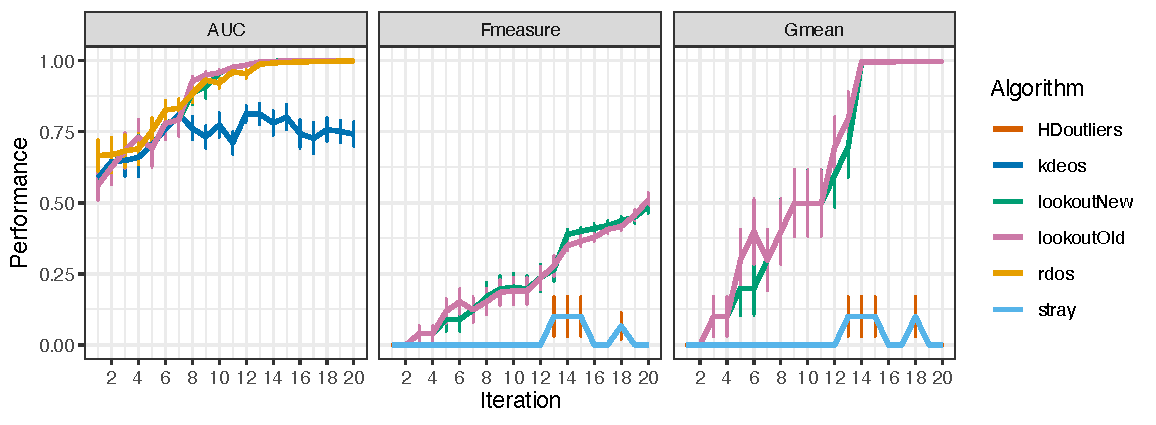
\includegraphics[width=\linewidth]{Figures/Experiment7_Comparison.pdf}
	\caption{Experiment 7 results}
	\label{fig:comparisonExp7}
\end{figure}

\subsection{Real-world Examples}

\subsubsection{Old-faithful dataset}

\begin{figure}[!ht]
	\centering
	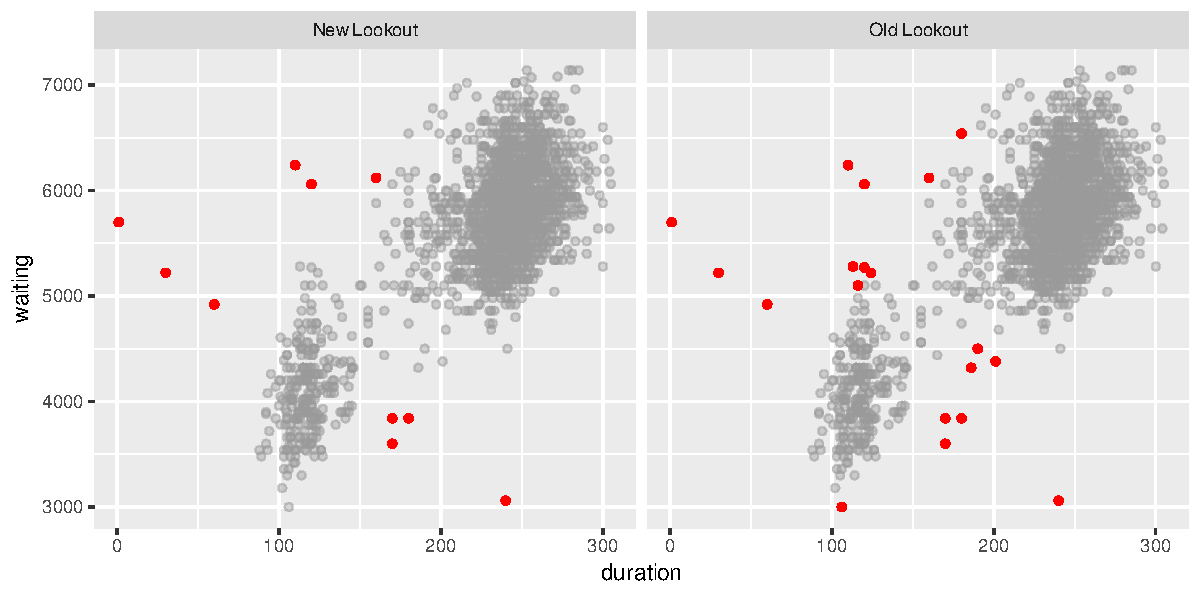
\includegraphics[width=\linewidth]{Figures/old_faithful.pdf}
	\caption{Anomalies in Old-Faithful dataset}
	\label{fig:oldfaithful}
\end{figure}


\subsubsection{Wine-reviews dataset}

\begin{figure}[!ht]
	\centering
	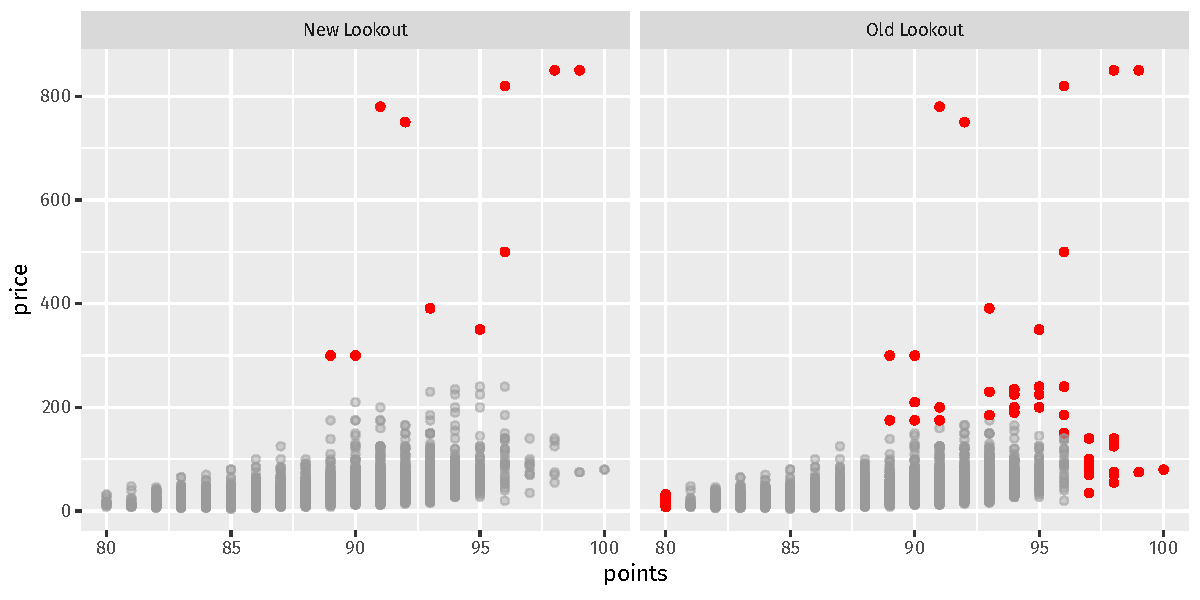
\includegraphics[width=\linewidth]{Figures/wine_reviews.pdf}
	\caption{Anomalies in Wine Reviews dataset}
	\label{fig:winereviews}
\end{figure}

\SK{Wine reviews is better than old-faithful dataset. All experiments are with shape\_zero = TRUE. }
